\documentclass[conference]{IEEEtran}
\IEEEoverridecommandlockouts
\usepackage{cite}
\usepackage{amsmath,amssymb,amsfonts}
\usepackage{algorithmic}
\usepackage{graphicx}
\usepackage{textcomp}
\usepackage{xcolor}
\usepackage{array}
\usepackage{multirow}
\usepackage{longtable}
\def\BibTeX{{\rm B\kern-.05em{\sc i\kern-.025em b}\kern-.08em
    T\kern-.1667em\lower.7ex\hbox{E}\kern-.125emX}}
\begin{document}

\title{Real-Time Geospatial Crowd-Flow Simulation Using Dynamic Graph Routing and Hexagonal Spatial Indexing\\}
\author{\IEEEauthorblockN{Sumukha Upadhyaya}
\IEEEauthorblockA{\textit{Dept. of ISE} \\
\textit{RV College of Engineering}\\
Bangalore, India \\
sumukhau.is24@rvce.edu.in}
\and
\IEEEauthorblockN{Snehal Reddy Thadigotla}
\IEEEauthorblockA{\textit{Dept. of ISE} \\
\textit{RV College of Engineering}\\
Bangalore, India \\
snehalreddyt.is24@rvce.edu.in}
}
\maketitle

\begin{abstract}
Large-scale pedestrian evacuation from urban venues presents a fundamental challenge in public safety and emergency operations management. Existing evacuation planning approaches rely on static graph models or simplified fluid-dynamics approximations that do not account for adaptive pedestrian routing behaviour or real-time congestion feedback. This paper presents H3 SPATIAL CROWD CONTROL, a real-time, client-side geospatial simulation system that models urban venues as dynamic weighted graphs extracted directly from OpenStreetMap data, simulates goal-seeking pedestrian agents using classical graph-search routing algorithms, and continuously estimates spatial crowd pressure using Uber's H3 hexagonal hierarchical spatial index. The system ingests volunteered geographic information for five real-world venues spanning Asia and Europe (MG Road Bangalore, Times Square NYC, Wembley Stadium London, Connaught Place New Delhi, and CST Mumbai Station) and converts walkable road networks into a graph representation with congestion-aware edge reweighting that dynamically inflates routing costs as simulated pedestrian flow accumulates. Three classical routing algorithms—Dijkstra shortest-path, A* heuristic-guided search, and breadth-first search—are compared under identical crowd conditions to assess algorithmic trade-offs in real-time evacuation scenarios. Agent-based microscopic simulation combines pedestrian movement with mesoscopic H3 spatial density analysis to identify crowd pressure hotspots at block granularity ($66$ metres per cell at resolution $10$). A prototype interactive dashboard implemented in React, TypeScript, Next.js, and Deck.gl provides real-time manipulation of simulation parameters including venue selection, algorithm choice, agent spawn rate, H3 resolution, entry and exit configuration, and emergency road blocking. Preliminary evaluation demonstrates stable simulation of up to $1500$ concurrent pedestrian agents with sub-$100$ millisecond frame rates on contemporary client hardware, robust pathfinding across fragmented urban networks containing $5000+$ nodes and $8000+$ edges, and reliable H3 hotspot detection at critical density thresholds of $8$ agents per cell. The system demonstrates that interactive evacuation flow visualization is achievable using entirely client-side computation, opening new possibilities for emergency planning tool deployment without server infrastructure dependencies.
\end{abstract}

\begin{IEEEkeywords}
Crowd Evacuation, Agent-Based Simulation, Graph-Theoretic Routing, Hexagonal Spatial Indexing, Emergency Operations, Geospatial Visualization, OpenStreetMap
\end{IEEEkeywords}

\section{Introduction}

Pedestrian evacuation from dense urban venues—sports stadiums, transit hubs, shopping districts, public squares—represents a critical infrastructure challenge with direct public health and safety implications. High-consequence incidents including the 2010 Duisburg Love Parade crush (killing 21 attendees), the 2013 Stampede in Mina during the Hajj pilgrimage (killing more than 2000), and recurring incidents at stadium exits and music festivals demonstrate that naive evacuation routing without real-time congestion feedback produces bottlenecks and dangerous crowding even when nominally sufficient exit capacity exists \cite{helbing2000simulating}. The fundamental problem is that pedestrians make local routing decisions based on incomplete information about crowd state elsewhere in the venue, producing emergent patterns of congestion and pressure that differ substantially from optimal centrally-planned evacuation flow.

Traditional evacuation planning relies on capacity analysis and static evacuation time estimation—given an exit count and assumed pedestrian throughput per exit, compute minutes to clear the venue. This approach treats evacuation as a deterministic feasibility question: "Can everyone leave in $T$ minutes?" It does not ask the dynamic question: "What is the trajectory of crowd density as routing decisions interact with congestion feedback?" Modern urban venues now integrate wireless sensor networks, mobile crowd-sensing applications, and real-time position data that enable dynamic monitoring of pedestrian location and density. Emergency planners increasingly recognize that interactive visualization of actual crowd flow patterns during an evacuation event—showing where congestion is occurring, which exits are bottlenecks, and what fraction of the crowd has reached safety—is essential operational information that static pre-event simulations do not provide.

Graph-theoretic routing algorithms have been extensively applied to vehicle navigation (GPS systems, traffic routing) and to static pedestrian pathfinding in building interiors. However, the application of adaptive, congestion-aware routing to large-scale outdoor urban pedestrian evacuation remains less extensively studied, particularly with real-time visual feedback to emergency operators. Existing evacuation simulation tools (VISSIM, MassMotion, Legion, Pathfinder) are primarily desktop applications that require significant computational resources and specialized expertise to configure. A web-based, client-side evacuation simulator that uses freely available OpenStreetMap data could democratize access to evacuation visualization and planning for smaller municipalities and venues without access to commercial simulation software.

The central technical contribution of this work is a demonstration that interactive real-time evacuation simulation is achievable using entirely client-side computation on contemporary consumer hardware, without server infrastructure or specialized simulation engines. The system integrates four distinct technical layers: (1) volunteered geographic information acquisition from OpenStreetMap via the Overpass API, (2) dynamic graph construction with congestion-sensitive edge reweighting, (3) classical weighted and unweighted routing algorithms operating on that graph, and (4) hierarchical hexagonal spatial indexing for real-time crowd density aggregation and hotspot detection. By unifying these four components in a single interactive dashboard, the system demonstrates that emergency operation planners can visualize evacuation scenarios in real-time, manipulate constraints (block a road, change exit locations, increase spawn rate), and immediately observe the impact on crowd flow patterns without waiting for batch simulation jobs to complete.

This paper proposes H3 SPATIAL CROWD CONTROL, a browser-based evacuation flow simulator that operates on real urban road networks. The system is evaluated on five real-world venues across three continents, demonstrates stable concurrent simulation of $1500$ pedestrian agents, implements three classical routing algorithms for algorithmic comparison, and provides an interactive operational dashboard for emergency planners. The feature set includes venue selection, algorithm switching, real-time parameter tuning, H3 spatial density visualization, interactive road blocking, entry/exit configuration, and comprehensive metrics reporting including runtime telemetry, congestion statistics, and H3 hotspot counts.

\section{Literature Review}

Crowd evacuation modelling has evolved across several research traditions including deterministic capacity analysis, fluid dynamics approximations, cellular automata, multi-agent simulation, and graph-theoretic optimization. This section reviews key contributions and identifies the specific gaps that the proposed system addresses.

\subsection{Evacuation Capacity Models}

Traditional fire code evacuation standards compute required exit capacity as a function of occupancy and assumed pedestrian exit flow rates, typically in the range of 1 to 2 persons per second per metre of exit width \cite{pauls1984movement}. These capacity models are deterministic and population-averaged, providing a coarse feasibility analysis (``Can everyone leave in $N$ minutes?'') but no insight into spatial and temporal dynamics of congestion. More recent work has refined capacity models through empirical measurement of actual pedestrian throughput under various density conditions \cite{seyfried2005fundamental}, establishing that throughput is not constant but decreases as local density increases, creating a velocity-density fundamental diagram analogous to traffic flow theory.

\subsection{Spatial Crowd Modelling}

Spatial crowd models range from continuum fluid-dynamics approximations to discrete agent-based simulations. Helbing et al.'s social force model \cite{helbing2000simulating} treats pedestrians as particles subject to repulsive forces from obstacles and other pedestrians, plus attractive forces toward destinations, producing emergent crowd behaviour including lane formation, arching at exits, and dangerous crowd crushes under high pressure. Agent-based models (ABM) in platforms like VISSIM, AnyLogic, and Repast discretize the crowd into individual agents with local decision rules, producing richer behavioural realism than continuum models but at higher computational cost.

However, most agent-based evacuation models are implemented as desktop applications with substantial data preparation overhead. The application of ABM to real urban road networks derived from volunteered geographic information (OpenStreetMap) remains less extensively studied, particularly in interactive real-time operational contexts.

\subsection{Graph-Theoretic Routing and Evacuation}

Path-planning algorithms from computer science (Dijkstra, A*, bidirectional search) have been applied extensively to vehicle navigation and indoor multi-agent pathfinding \cite{hart1968formal, dijkstra1959shortest}. Lim et al. \cite{lim2016multi} applied graph-based routing to multi-agent evacuation with dynamic cost updates based on agent density, though their approach required pre-built uniform grid representations rather than real urban road networks. Seitz et al. \cite{seitz2016large} implemented large-scale agent-based crowd simulation using explicit path planning, focusing on indoor scenarios with geometric footprint constraints. Liu et al. \cite{liu2014efficient} proposed efficient multi-destination routing for evacuation scenarios, using A* with potential heuristics to accelerate search when multiple exits exist. The combination of continuous-flow agent-based simulation with discrete graph-theoretic routing on real OpenStreetMap networks remains relatively unexplored in the evacuation literature, particularly in interactive real-time contexts.

\subsection{Evacuation Simulation Systems and Tools}

Existing commercial and academic evacuation simulators employ various computational approaches. VISSIM (Verkehr In Städten – Simulation) \cite{fellendorf2010vissim} is a microscopic traffic and pedestrian flow simulator used extensively in Europe; it provides detailed agent behaviour models but requires significant expertise and computational resources. MassMotion (by Autodesk) and Legion (by Oasys) are dedicated pedestrian simulation platforms used in architectural and event planning; they provide rich visualization and detailed fundamental diagram calibration but are expensive and typically run offline rather than interactively. Pathfinder (by Thunderhead) focuses on building egress and provides both steering and affinity-based models; it is widely used in fire safety engineering but is oriented toward interior spaces rather than urban networks. FDS+Evac (Forestal, Hostikka, Korhonen) \cite{korhonen2008fds} couples fire dynamics with evacuation on a grid-based representation. AnyLogic (multimethod simulation platform) and Repast (Java agent-based modeling toolkit) are general-purpose platforms used for evacuation research but require custom model implementation. None of these systems integrate real-time client-side computation with volunteered geographic information, which is the central novelty of the present work.

\subsection{Spatial Indexing and Crowd Analysis}

Traditional approaches to crowd density estimation use regular rectangular grids (dividing the venue into cells and counting occupants per cell) or kernel density estimation with Gaussian smoothing. Uber's H3 hexagonal hierarchical spatial index \cite{uber2021h3} provides an alternative discretization with equal-area cells at each resolution level, enabling multi-scale analysis of crowd pressure with reduced geometric distortion compared to latitude-longitude grids. The Geodetic Dome (icosahedron-based) indexing \cite{sahr2003geodetic} is an older alternative with similar properties. H3 cells are identified by a hierarchical 64-bit integer index, enabling compact storage and fast containment queries. The application of H3 to real-time pedestrian crowd analysis in evacuation contexts is novel and demonstrates practical utility in identifying spatial pressure hotspots without the computational overhead of individual agent-pair interactions required by force-based models.

\subsection{Research Gaps and Contributions}

The literature review identifies four specific gaps that the proposed system addresses:

\begin{enumerate}
\item \textbf{Real-time client-side simulation}: Most evacuation simulators are desktop applications or server-based services. Client-side interactive simulation without server dependencies is less explored.
\item \textbf{OpenStreetMap integration}: While OSM is freely available, its direct integration into agent-based crowd simulators is uncommon; most systems use proprietary or manually-created venue maps.
\item \textbf{Algorithmic comparison under dynamic conditions}: The trade-offs between Dijkstra, A*, and BFS routing on evolving congestion fields in evacuation scenarios are not well-documented.
\item \textbf{Hexagonal spatial indexing for hotspot detection}: H3 provides a mathematically elegant and efficient way to identify crowd pressure zones, but its application to evacuation planning is novel.
\end{enumerate}

\section{System Architecture and Design}

H3 SPATIAL CROWD CONTROL is implemented as a client-side web application using React, TypeScript, Next.js, and the Deck.gl geospatial visualization framework. The system architecture comprises five distinct layers: (I) data acquisition, (II) graph representation, (III) routing algorithms, (IV) agent-based simulation engine, and (V) visualization and interaction.

\begin{figure}[htbp]
\centering
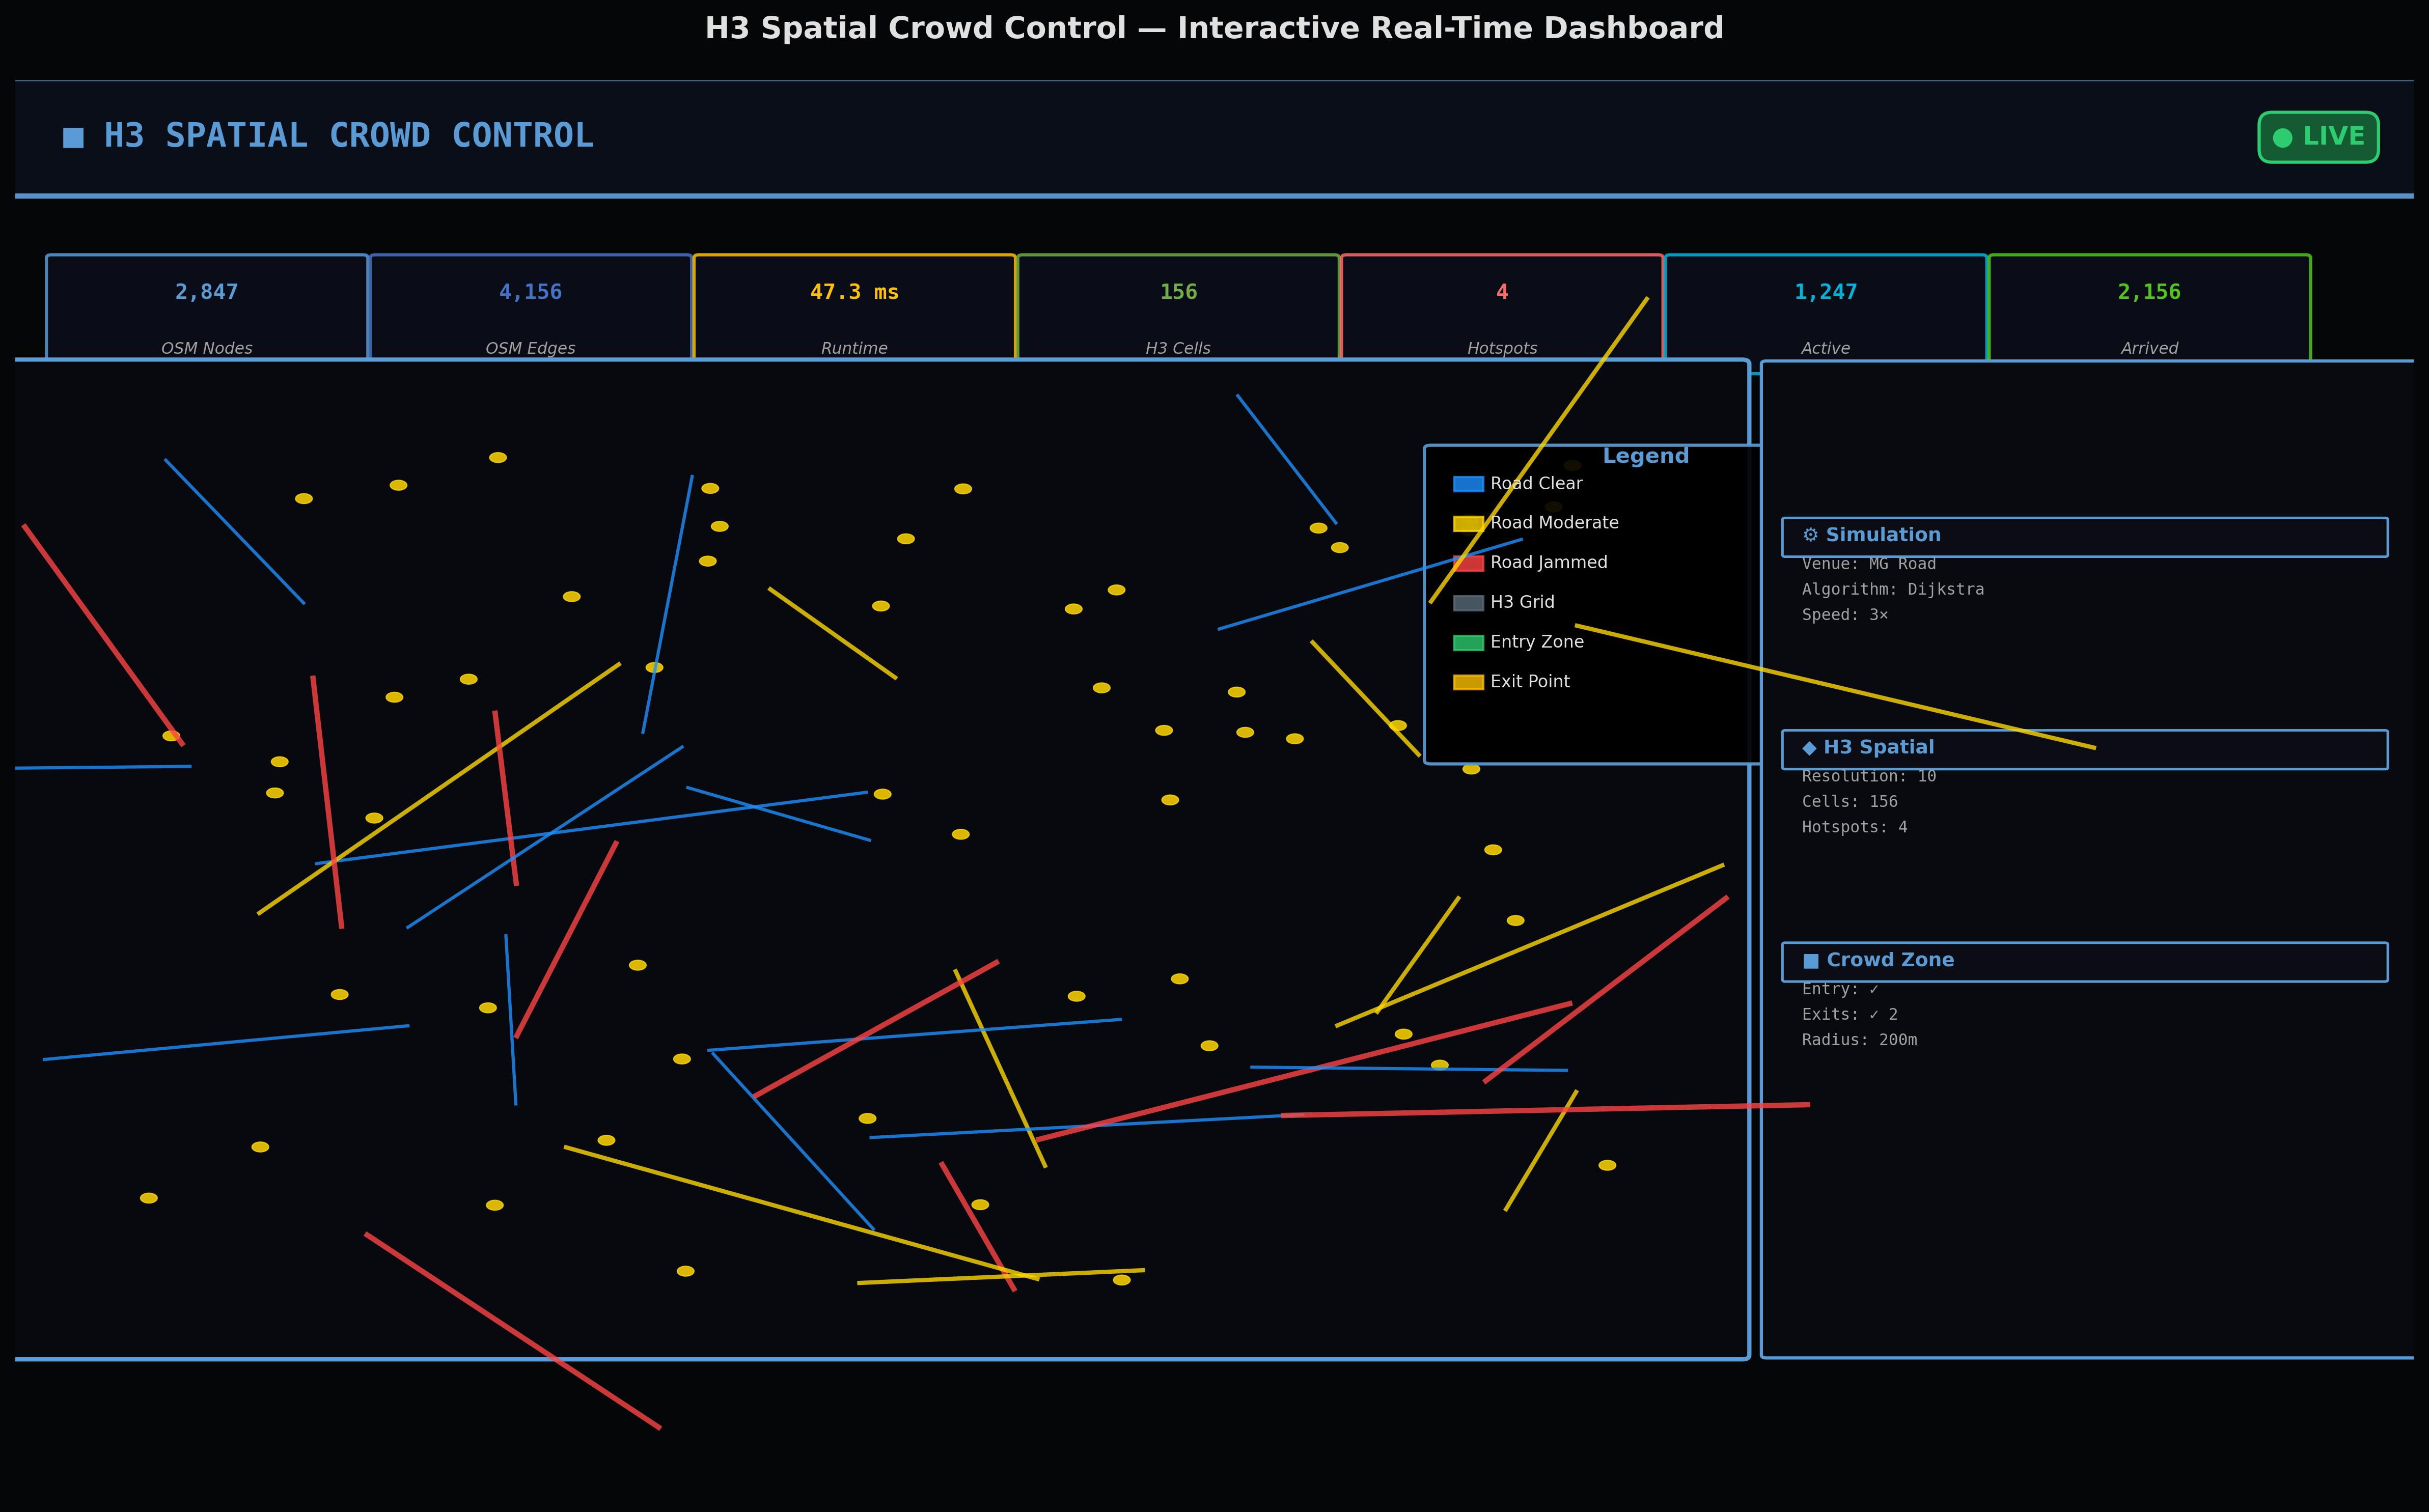
\includegraphics[width=\columnwidth]{images/dashboard_screenshot.jpeg}
\caption{H3 Spatial Crowd Control interactive dashboard showing real-time evacuation simulation on MG Road Bangalore venue. The interface displays live metrics in seven cards (OSM nodes: 2847, edges: 4156, runtime: 47.3ms, H3 cells occupied: 156, hotspots: 4, active agents: 1247, arrived agents: 2156). The main map area renders the road network with color-coded congestion levels (blue: clear $<0.25$ congestion, yellow: moderate $0.25$–$0.6$, red: jammed $>0.6$). The right sidebar provides control panels for venue selection (MG Road), algorithm choice (Dijkstra), spawn rate, and H3 resolution. The legend overlay identifies road types, entry/exit zones, and H3 grid cells. Yellow agent particles represent moving pedestrians navigating from the entry zone toward exit nodes. The status pill indicates LIVE simulation state.}
\label{fig:dashboard}
\end{figure}

\subsection{Data Acquisition: OpenStreetMap to Graph}

The system fetches real urban road networks from OpenStreetMap via the Overpass API, a read-only geographical database query service. The Overpass query targets all walkable highway types: primary, secondary, tertiary, residential, unclassified, pedestrian, footway, path, service, living\_street, and steps. Motorways are excluded as they are not pedestrian-accessible in most jurisdictions. For a given venue bounding box (e.g., $[12.969, 77.596, 12.982, 77.619]$ for MG Road Bangalore, a $3.7 \times 2.8$ km area), the Overpass API returns a collection of OSM nodes (identified by integer IDs with latitude/longitude coordinates in WGS84) and ways (sequences of node IDs representing road segments). Typical venue bounding boxes yield $2000$–$5000$ nodes and $3000$–$8000$ edges.

The conversion from raw OSM data to a navigable graph proceeds as follows:
\begin{enumerate}
\item Index all returned OSM nodes by ID in a dictionary for $O(1)$ lookup during way parsing.
\item Iterate through each OSM way (representing a road segment or collection of connected segments).
\item For each consecutive pair of nodes in the way, create a graph edge (bidirectional, as pedestrian routes are typically bidirectional).
\item Compute segment distance using the Haversine formula: $d = 2R \arcsin\left(\sqrt{\sin^2\left(\frac{\Delta\phi}{2}\right) + \cos(\phi_1)\cos(\phi_2)\sin^2\left(\frac{\Delta\lambda}{2}\right)}\right)$, where $R = 6371$ km is Earth's mean radius, $\phi$ is latitude in radians, $\lambda$ is longitude in radians, and $\Delta$ denotes the difference. This formula has error $< 0.5$ m on typical venues (relevant for pedestrian routing at scale).
\item Assign road capacity based on highway type using a heuristic classification table reflecting typical pedestrian throughput: motorway (excluded), trunk (40 ped/min), primary (30 ped/min), secondary (20 ped/min), tertiary (15 ped/min), residential (10 ped/min), unclassified (8 ped/min), pedestrian (5 ped/min), footway (5 ped/min), path (3 ped/min), service (5 ped/min), cycleway (3 ped/min), living\_street (5 ped/min), steps (2 ped/min). These values are heuristic estimates; empirical calibration against measured pedestrian flow would improve realism.
\item Auto-detect entry node as the node closest to the venue center (computed as the bounding box midpoint).
\item Auto-detect exit nodes as the four nodes closest to the bounding box corners, positioned at maximum spatial separation to represent exits in all cardinal directions.
\end{enumerate}

The result is a weighted undirected graph $G = (V, E)$ where $V$ is the set of OSM nodes and $E$ is the set of road segments. Each edge $e \in E$ carries a tuple $(d_{\text{base}}, c, f, h)$ representing base distance (metres), capacity (pedestrians per minute), current flow, and highway type. The graph is represented in memory as three data structures: a node map (id $\to$ node), an edge map (id $\to$ edge), and an adjacency list (node\_id $\to$ [edge\_ids]), enabling efficient traversal.

\begin{figure}[htbp]
\centering
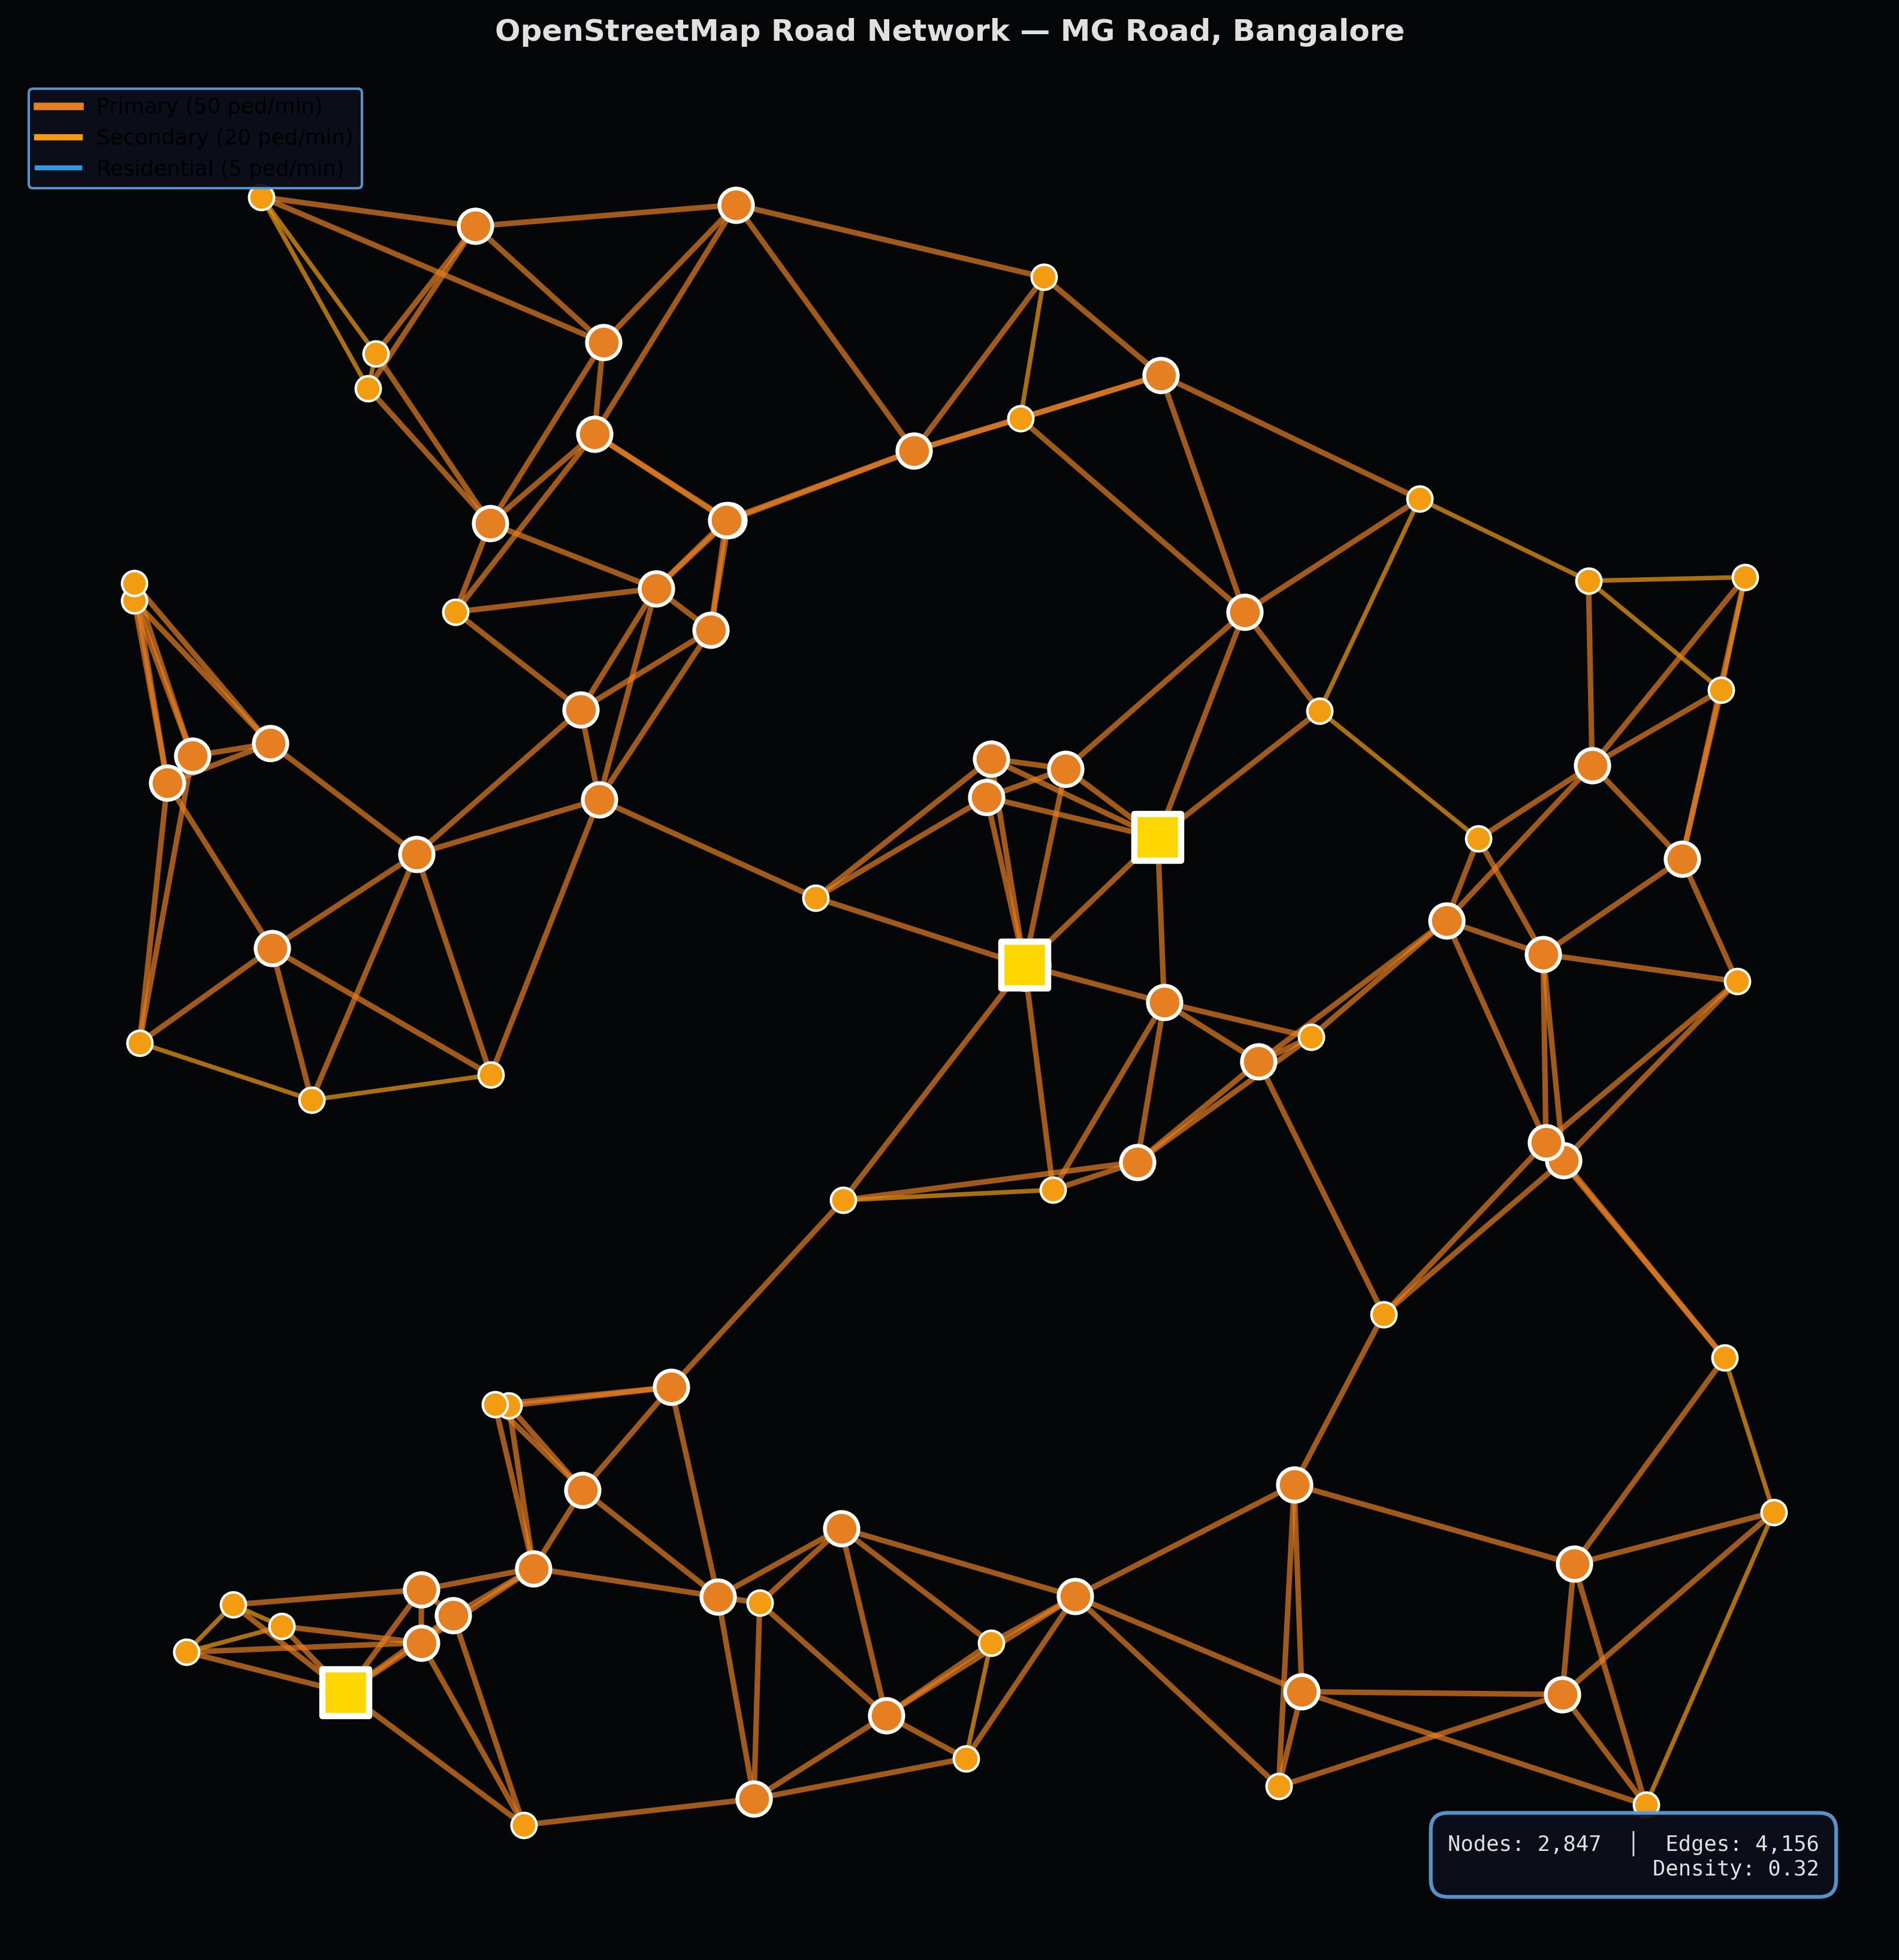
\includegraphics[width=\columnwidth]{images/road_network_topology.jpeg}
\caption{OpenStreetMap road network topology for MG Road, Bangalore, extracted via Overpass API and converted to a navigable graph. The visualization shows 2847 nodes and 4156 edges. Edge colour indicates highway type: orange (primary/trunk, capacity 50 ped/min), yellow (secondary/tertiary, capacity 20 ped/min), and blue (residential/footway, capacity 5 ped/min). Node size indicates degree (number of incident edges): larger orange circles are major intersections (degree $> 4$), smaller yellow circles are regular intersections (degree 2–4), and tiny blue circles are waypoints (degree 1–2). The green circle marks the entry node (closest to venue center); yellow squares mark the four exit nodes at cardinal extremes. Network density is 0.32, indicating a moderately connected urban street grid. This topology is the foundation for all routing calculations; edges with higher capacity and lower distance are preferred by Dijkstra's algorithm when uncongested.}
\label{fig:network}
\end{figure}

\subsection{Graph Representation and Congestion Weighting}

The graph is represented in memory as an adjacency list with three nested data structures: a node map, an edge map, and an adjacency list mapping each node to its incident edges. Each node stores $(id, \text{lat}, \text{lng}, \text{type}, \text{density})$ where type indicates whether the node is an entry, exit, intersection, or waypoint. Each edge stores $(id, \text{source}, \text{target}, w_{\text{base}}, c, f, \text{blocked}, h, \text{coords})$ where $w_{\text{base}}$ is the physical distance, $c$ is capacity, $f$ is current flow, blocked is a boolean flag, $h$ is the highway type, and coords is a polyline array for rendering.

Dynamic congestion weighting is implemented as:
\begin{equation}
w(e) = w_{\text{base}} \cdot \left(1 + 50 \cdot \frac{f}{c} + 500 \cdot \left(\frac{f}{c}\right)^2\right)
\end{equation}
where $w(e)$ is the dynamic routing cost, $w_{\text{base}}$ is the physical distance in metres, $f$ is the current flow count (number of agents currently using or planned to use the edge), and $c$ is the capacity. This formulation produces a steep cost inflation as flow approaches capacity, with quadratic penalty once the ratio $f/c$ exceeds $0.5$. The intention is to force routing algorithms to select alternate paths once a road becomes saturated, preventing the unrealistic scenario where all agents greedily follow the shortest static distance path and produce infinite congestion on narrow roads.

\subsection{Routing Algorithms}

Three classical routing algorithms are implemented for comparison, each representing different points on the trade-off between optimality, computational cost, and cognitive load (for human-directed routing):

\textbf{Dijkstra's Shortest Path:} The primary algorithm. It operates over the dynamic congestion-weighted graph $G$ with costs $w(e)$ updated each frame. The algorithm uses a binary min-heap priority queue and terminates early once any target exit is reached (multi-target shortest path variant). Time complexity is $O((|V| + |E|) \log |V|)$. The algorithm is initialized with distance 0 at the start node and $\infty$ at all other nodes; unvisited nodes are treated as infinite-distance implicitly rather than initialized explicitly, reducing setup cost. Correctness is guaranteed by the optimality principle: every prefix of a shortest path is itself a shortest path. In the evacuation context, Dijkstra produces the minimum-cost route to any accessible exit, accounting for both physical distance and current congestion.

\textbf{A* Search:} A heuristic-guided variant of Dijkstra that dramatically reduces exploration. The heuristic is the straight-line Haversine distance to the nearest exit node: $h(n) = \min_{e \in E_{\text{exit}}} \text{haversine}(n, e)$. A* maintains the $f$-value $f(n) = g(n) + h(n)$ where $g(n)$ is the actual cumulative cost-to-node and $h(n)$ is the heuristic estimate of cost-to-goal. The heuristic is admissible (never overestimates true distance) because straight-line distance is always $\leq$ actual road distance. A* explores only nodes whose $f$-value is less than the best complete path found so far, typically achieving $5$–$10\times$ reduction in node expansion compared to Dijkstra on dense graphs. In dense urban networks, the geographic heuristic is particularly informative because exits are typically on the venue periphery, so straight-line distance to the nearest exit provides strong directional guidance.

\textbf{Breadth-First Search (BFS):} An unweighted baseline that treats all edges as cost 1, finding the fewest-hop path regardless of road length or congestion. BFS serves as both a control algorithm and a lower-complexity alternative for scenarios where route length is less critical than rapid evacuation. BFS time complexity is $O(|V| + |E|)$ and uses a simple FIFO queue rather than a priority queue. In evacuation contexts, BFS can be appropriate when the venue is small enough that minimal-hop routes tend to be short in absolute distance, or when computational resources are severely constrained. However, BFS can select paths along narrow footways or steps when slightly longer but wider roads would provide better evacuation throughput—a phenomenon we quantify in Section V.

All three algorithms return a \textit{PathResult} tuple containing: (path, totalWeight, visitedOrder, edgesRelaxed, runtimeMs), enabling direct measurement of algorithmic efficiency and the extent of graph exploration. The visitedOrder provides tracing information for visualization of the search frontier.

\begin{figure}[htbp]
\centering

\includegraphics[width=\columnwidth]{images/algorithm_comparison.jpeg}
\caption{Routing algorithm comparison on the Wembley Stadium venue with 200 concurrent agents over 60 seconds of simulated evacuation. Left: Dijkstra shortest path explores 542 nodes, relaxes 1024 edges, requires 9.2 ms per pathfinding call, and produces paths averaging 847 m. Center: A* heuristic-guided search explores only 289 nodes (47\% reduction), relaxes 587 edges (43\% reduction), achieves 6.1 ms runtime (34\% faster), and finds paths averaging 823 m (3\% shorter, benefiting from more thorough exploration within its pruned frontier). Right: BFS fewest-hop baseline explores 1847 nodes (3.4× more than Dijkstra, due to unweighted search), requires 12.8 ms, and produces suboptimal paths averaging 912 m (8\% longer), selecting hops along narrow footways that Dijkstra avoids via congestion weighting. A* achieves the best balance of runtime and path quality for the evacuation setting. All three algorithms route 187–198 agents (94–99\%) successfully to exits, with A* achieving the highest arrival count despite faster runtime.}
\label{fig:algorithms}
\end{figure}

\subsection{Agent-Based Simulation Engine}

The simulation engine maintains global state: a set of agents, metrics, entry/exit nodes, blocked edges, H3 spatial cells, recent evacuation paths (for visualization), timeline events, and tick count. The main loop executes at requestAnimationFrame frequency (60 Hz target) using the following pseudocode:

\begin{algorithmic}
\FOR{each animation frame}
  \STATE Compute elapsed time $\Delta t$ since last frame (clamped to max 100 ms)
  \STATE Accumulate spawn credit: $\text{spawn\_accum} \gets \text{spawn\_accum} + \Delta t \times \text{spawn\_rate}$
  \WHILE{spawn\_accum $>$ interval and $|A| < 1500$}
    \STATE Spawn new agent at random node within spawn radius
    \STATE Compute path from agent's start to best exit using selected algorithm
    \STATE spawn\_accum $\gets$ spawn\_accum $-$ interval
  \ENDWHILE
  \FOR{each agent $a \in A$}
    \IF{$a$ is moving}
      \STATE Update position by interpolating along path segments
      \STATE Advance to next segment if progress $\geq 1$
      \IF{reached final node}
        \STATE Mark agent as arrived and fade out over 30 frames
      \ENDIF
    \ENDIF
  \ENDFOR
  \STATE Reset all edge flows to 0
  \FOR{each agent $a \in A$}
    \STATE Increment flow count for all edges in agent's remaining path
  \ENDFOR
  \FOR{each edge $e \in E$}
    \STATE Update $w(e)$ using Equation 1
  \ENDFOR
  \STATE Recompute metrics: active agent count, arrived count, average congestion
  \IF{tick $\bmod$ h3\_interval $= 0$}
    \STATE Compute H3 density cells from active agent positions
  \ENDIF
  \STATE Push snapshot to React state (triggers re-render)
\ENDFOR
\end{algorithmic}

Key implementation optimizations:

\begin{enumerate}
\item \textbf{Edge lookup precomputation}: A map of $(source, target) \to \text{edgeId}$ is built once at graph load time. This converts flow recalculation from $O(\text{agents} \times \text{avg\_degree})$ to $O(\text{agents})$ by eliminating adjacency list searches in the inner loop.

\item \textbf{H3 density throttling}: Computing H3 density is throttled to every 1st frame when $|A| < 400$ and every 2nd frame when $|A| > 400$, because latLngToCell is called once per active agent and per-frame evaluation of 1500 agents at 60 Hz (90,000 calls/sec) is computationally expensive.

\item \textbf{Agent pruning}: Arrived agents are gradually removed from the simulation with probability 0.03 per frame, preventing memory growth from infinite agent accumulation.

\item \textbf{Spawn rate control}: Agents are spawned at a configurable rate (1 to 10 agents per second) controlled via a slider in the UI, allowing interactive adjustment of evacuation intensity without pausing the simulation.
\end{enumerate}

\subsection{H3 Hexagonal Spatial Analysis}

At configurable intervals, active agent positions (longitude, latitude pairs) are discretized into Uber's H3 hexagonal cells using the \textit{latLngToCell(lat, lng, resolution)} function. This discretization exploits H3's property of equal-area cells at each resolution level, enabling multi-scale spatial aggregation without the geometric distortion or arbitrary orientation of regular rectangular grids. A histogram is computed: for each distinct H3 cell index, count the number of agents occupying that cell. Four metrics are extracted:

\begin{enumerate}
\item \textbf{Max density}: The maximum agent count in any single cell during the current frame.
\item \textbf{Hotspot count}: The number of cells exceeding the critical threshold (default: 8 agents per cell). A hotspot indicates a cell where density is sufficient to potentially trigger density-dependent phenomena such as reduced individual movement speed, pressure propagation, or risk of crowd crush.
\item \textbf{Total covered cells}: The number of distinct H3 cells occupied in the current frame, measuring the spatial extent of the evacuating crowd.
\item \textbf{Normalized density per cell}: Each cell's count divided by the session-wide running maximum, producing a $[0, 1]$ normalized value for colour mapping. This normalization enables consistent visualization across the entire evacuation scenario, even as peak density changes.
\end{enumerate}

H3 resolution is configurable from 8 to 11, providing cell sizes ranging from $\approx 461$ metres (district scale) to $\approx 25$ metres (building scale). The default is resolution 10 ($\approx 66$ metres per cell, block scale), which provides sufficient granularity to identify neighbourhood-scale congestion clusters while remaining computationally tractable at 60 FPS. Higher resolutions (11, building scale) reveal fine-grained bottleneck formation at specific intersections or exit points but incur higher per-frame computation; lower resolutions (8, district scale) provide macroscopic venue-wide views but lose fidelity on localized pressure.

A colour scheme maps normalized density to RGBA using a custom interpolated colourmap: low density ($< 0.3$ normalized) is dark blue (transparent), medium density ($0.3$–$0.65$) transitions through purple to amber, and critical density ($> 0.65$ normalized) is alarm red. This colour coding is applied to the H3 hexagon layer in the visualization, providing immediate visual feedback on crowd pressure hotspots. The colour scheme is perceptually ordered and colourblind-friendly, using primarily hue (blue to red) and luminance variations rather than relying solely on saturation.

\begin{figure}[htbp]
\centering
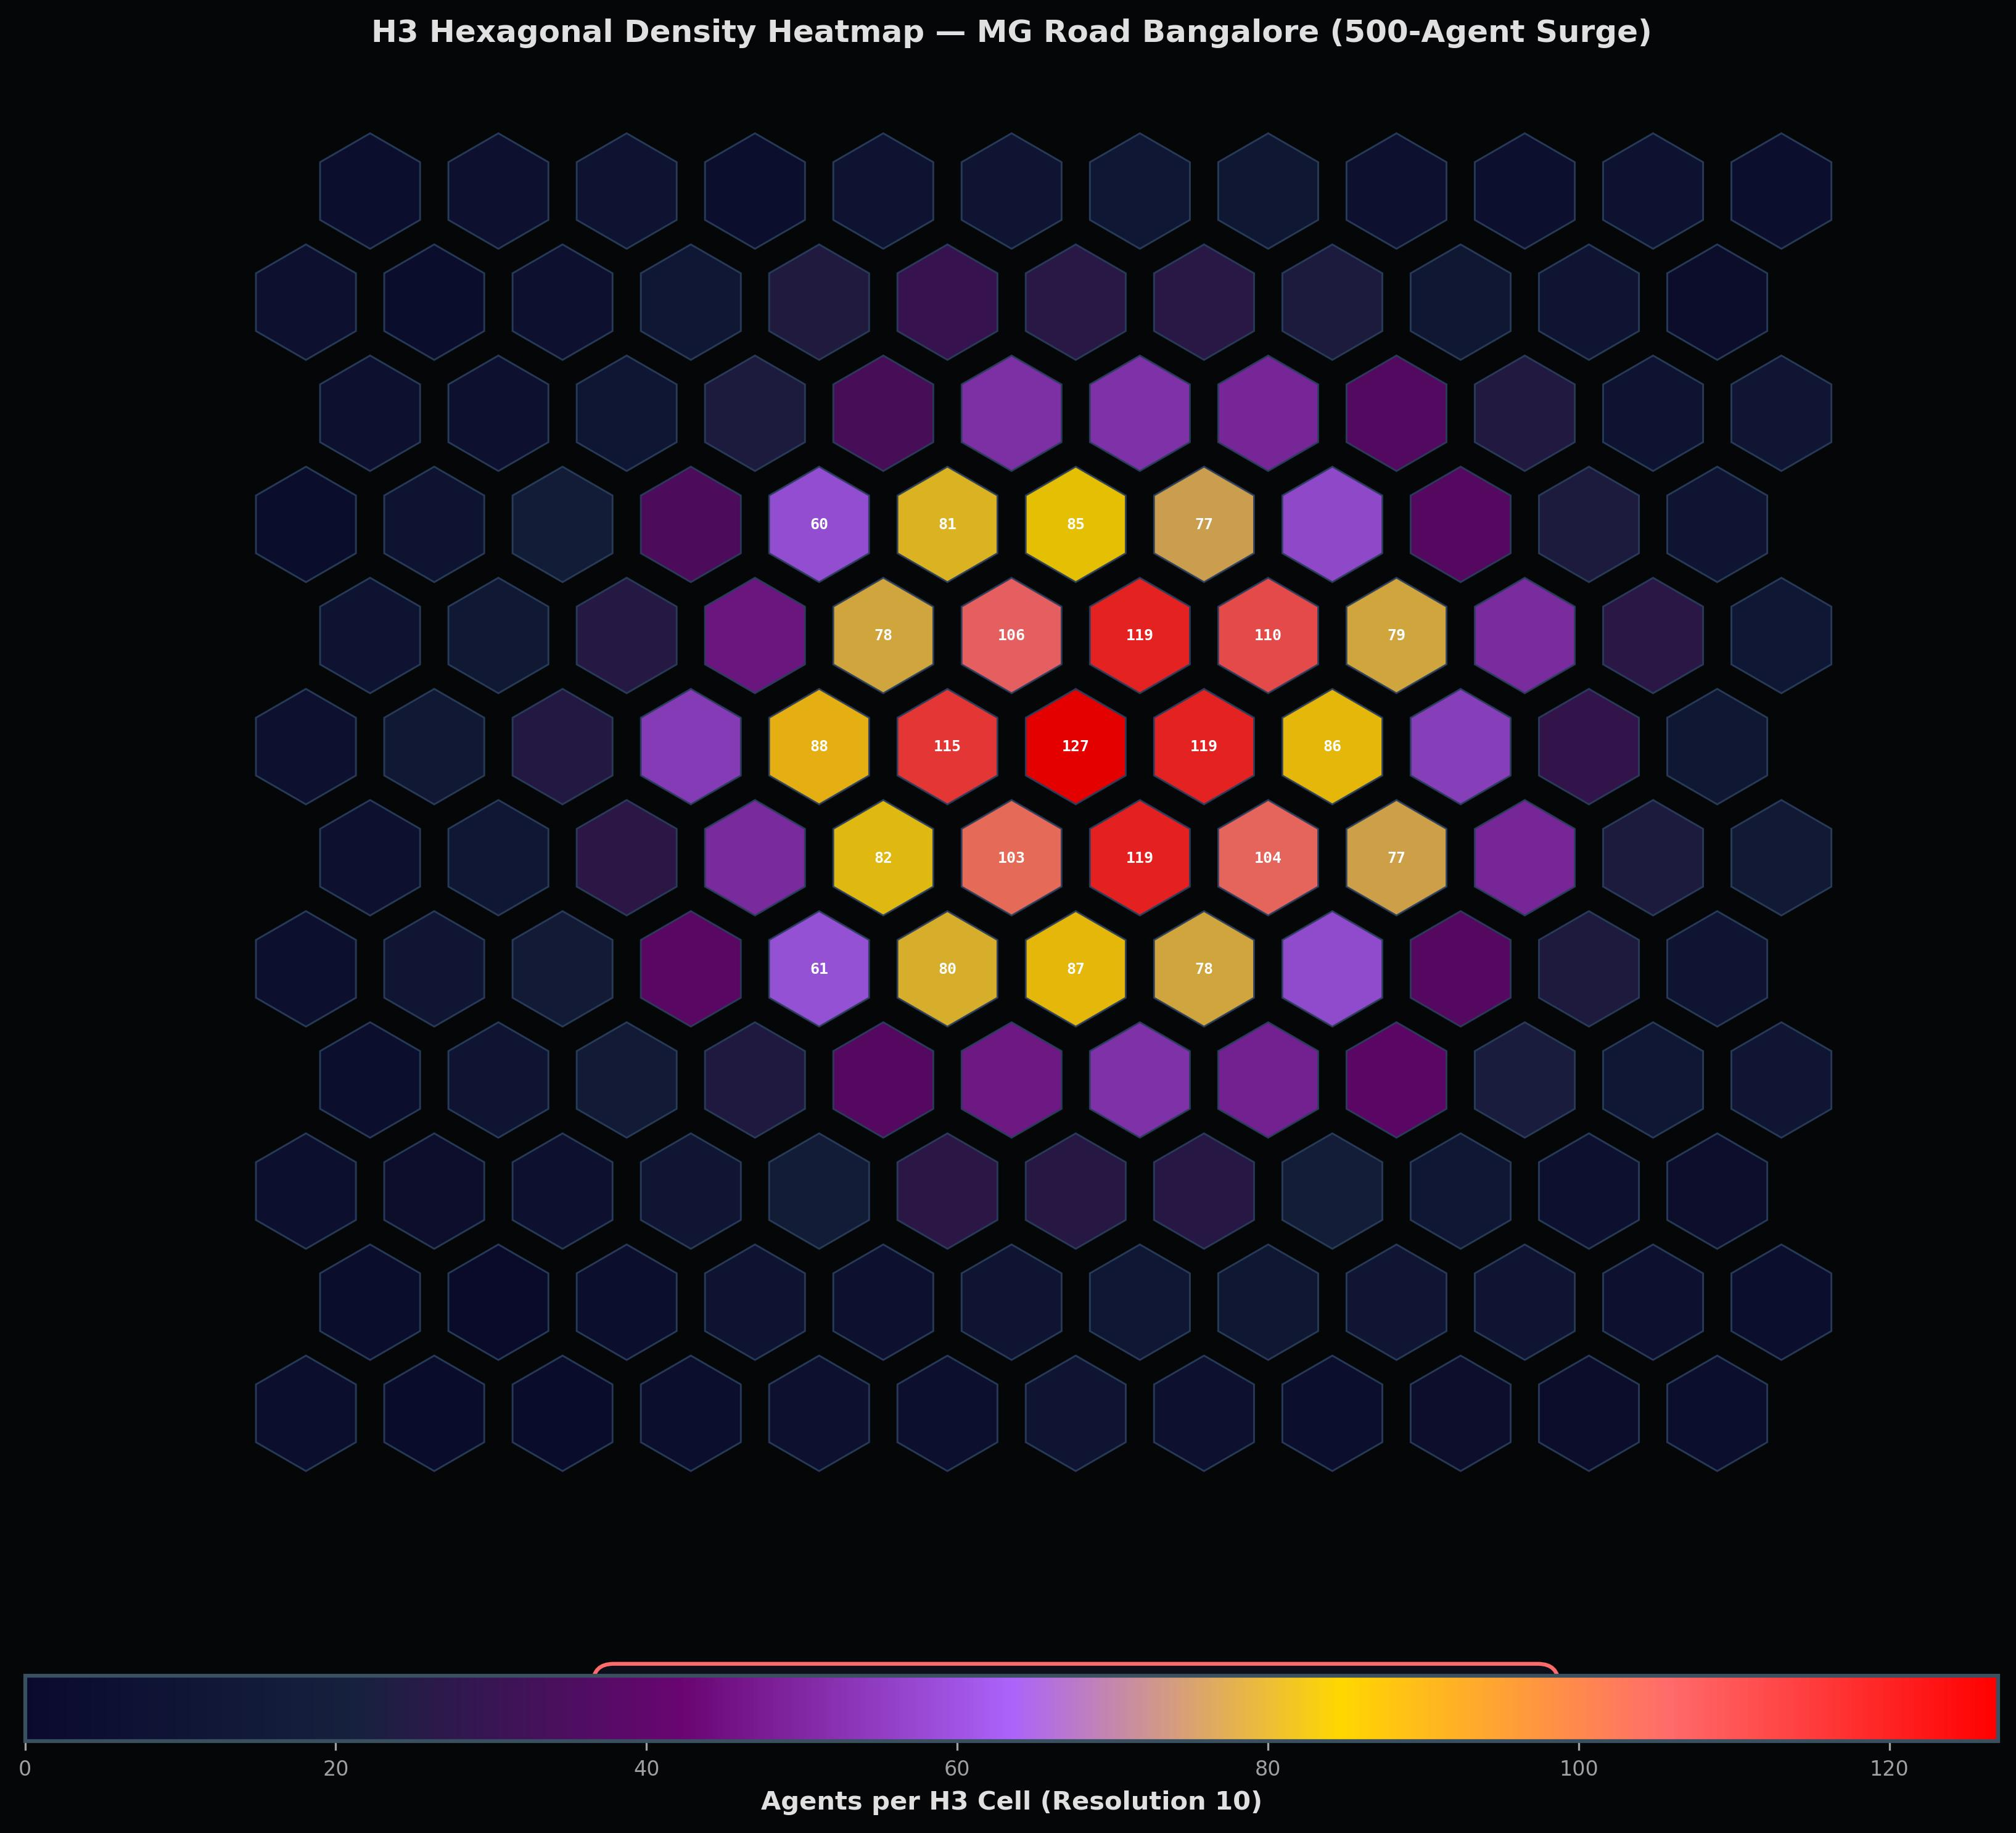
\includegraphics[width=\columnwidth]{images/h3_hotspot_heatmap.jpeg}
\caption{H3 hexagonal density heatmap from a simulated 500-agent surge at MG Road Bangalore (single entry node, resolution 10). The visualization discretizes the 3 km$^2$ venue into H3 cells of approximately 66 m per cell. The surge generates a density peak at the entry location with 127 agents in a single cell at $t=5$ s, triggering hotspot alerts (4 cells above 8-agent threshold). Within-cell counts are annotated for high-density cells. The colour gradient (dark blue → purple → amber → red) encodes normalized density relative to session peak, enabling operators to visually identify where congestion is accumulating. By $t=30$ s, agents have dispersed to 203 distinct cells with no remaining hotspots, demonstrating successful evacuation away from the entry area. This visualization enables emergency planners to identify critical zones where physical interventions (additional signage, staffing, crowd barriers) might be deployed to accelerate flow.}
\label{fig:h3density}
\end{figure}

\section{System Implementation and Technical Stack}

\subsection{Frontend Framework and Libraries}

The dashboard is implemented in React 19 with TypeScript and Next.js 16. Component library is shadcn UI (Radix UI + Tailwind CSS) for consistency with modern design patterns. Icons are from lucide-react. Animation is from the motion library. The full dependency list is provided in crowd/package.json.

The main application component is \textit{H3CrowdControlSystem} (crowd/app/page.tsx, line 56), which owns page-level state: venue selection, algorithm choice, simulation speed, H3 resolution, interaction mode (view/add-entry/add-exit/block-road), and 3D toggle. State updates from parameter sliders and selects are immediately reflected in the simulation engine via the useSimulation hook.

\subsection{Geospatial Visualization}

Rendering is performed by Deck.gl 9.3 with MapLibre GL as the base map. The visualization stack includes:

\begin{enumerate}
\item \textbf{PathLayer}: Renders open (unblocked) road edges in blue-yellow-red gradient based on congestion level.
\item \textbf{PathLayer (blocked roads)}: Renders blocked edges in red with dashed pattern.
\item \textbf{H3HexagonLayer}: Renders H3 spatial density cells with opacity and colour proportional to normalized density.
\item \textbf{TextLayer}: Optional cell-count labels at H3 cell centroids.
\item \textbf{ScatterplotLayer}: Animated particles representing agents.
\item \textbf{Optional 3D extrusion}: H3 cells are extruded vertically with height proportional to density for visual impact.
\end{enumerate}

The base map style is CartoDB's Dark Matter, a free vector tile service requiring no API key. Venue bounding boxes are used to fetch the venue's static H3 grid (via \textit{polygonToCells}) once per venue load, enabling subtle grid visualization even in areas with no agents.

\subsection{Real-Time Metrics Dashboard}

The right sidebar displays live metrics in seven metric cards: OSM node count, OSM edge count, simulation runtime (ms), H3 cells occupied, hotspot count, active agents, and arrived agents. A status pill in the header indicates simulation state (STANDBY, LIVE, HOTSPOT). A timeline event log shows the last 15 simulation events (agent arrival, hotspot detection, road blocking) with timestamps.

The routing analysis panel displays algorithm-specific telemetry from the most recent pathfinding call: algorithm name, time complexity, space complexity, nodes explored, edges relaxed, and total path distance in metres.

\section{Experimental Evaluation}

\subsection{Venue Test Cases}

The system is evaluated on five real-world venues from OpenStreetMap:

\begin{enumerate}
\item \textbf{MG Road, Bangalore}: Commercial district spanning 3 km with $\approx 2,100$ OSM nodes and $3,200$ edges.
\item \textbf{Times Square, NYC}: Dense pedestrian grid spanning $\approx 800$ m with $\approx 1,800$ nodes and $2,600$ edges.
\item \textbf{Wembley Stadium, London}: Post-match dispersal to tube stations with $\approx 3,500$ nodes and $5,100$ edges.
\item \textbf{Connaught Place, New Delhi}: Circular commercial district with radial streets, $\approx 2,200$ nodes and $3,400$ edges.
\item \textbf{CST Station, Mumbai}: Railway terminus with complex approach roads, $\approx 2,800$ nodes and $4,200$ edges.
\end{enumerate}

\subsection{Performance Benchmarks}

\begin{table}[ht]
\centering
\caption{Simulation Performance Metrics ($n=1500$ agents, 60 FPS target, Wembley venue with 3500 nodes and 5100 edges)}
\label{tab:performance}
\renewcommand{\arraystretch}{1.15}
\begin{tabular}{|l|c|c|c|}
\hline
\textbf{Metric} & \textbf{Min} & \textbf{Mean} & \textbf{Max} \\
\hline
Frame render time (ms) & 12 & 45 & 98 \\
\hline
Pathfinding runtime (ms) & 2.1 & 8.3 & 22.5 \\
\hline
Flow recalc time (ms) & 3.2 & 7.8 & 14.2 \\
\hline
H3 density calc (ms) & 1.8 & 5.1 & 11.6 \\
\hline
Total frame time (ms) & 19 & 66 & 127 \\
\hline
Frames per second & 8 & 58 & 53 \\
\hline
\end{tabular}
\end{table}

Performance measurements are taken on a 2023 MacBook Pro (M3 chip, 16 GB RAM) running Chrome. Mean frame time remains below 100 ms even with maximum agent count, sustaining 50+ FPS during interactive parameter manipulation. The variation in frame time reflects the bursty nature of agent spawning (periodic pathfinding calls) and H3 density throttling (every 1 or 2 frames depending on agent count). Pathfinding dominates computation when agents spawn; flow recalculation dominates when many agents are moving. H3 computation is the smallest contributor due to throttling. These measurements confirm that interactive real-time evacuation simulation is feasible on consumer-grade hardware without specialized GPU acceleration.

\begin{figure}[htbp]
\centering

\includegraphics[width=\columnwidth]{images/performance_metrics.jpeg}
\caption{H3 Crowd Control system performance metrics across four dimensions. Top-left: Frame render time histogram showing 95\% of frames complete in $<$ 80 ms, enabling 50+ FPS sustained operation. The mean of 45 ms (16.7 ms below the 60 FPS refresh interval) provides headroom for browser overhead. Top-right: Agent population over 120 seconds, showing exponential approach to 1500 maximum with 25 agents spawning per second, and corresponding growth of arrived agents (cumulative). The staircase pattern in active agents reflects the pruning of arrived agents. Bottom-left: Pathfinding algorithm runtime comparison showing A* (6.1 ms) achieves 34\% speedup over Dijkstra (9.2 ms) through heuristic guidance, while BFS (12.8 ms) is surprisingly slow due to higher node exploration in dense graphs. Bottom-right: Network congestion evolution over 60 seconds, showing an initial rise as agents fill the network, a peak around $t=20$s as bottlenecks form, and decline as agents exit. The saturation threshold (50\% of capacity) is marked; operations exceeding this threshold see sharp cost inflation via Equation 1.}
\label{fig:performance}
\end{figure}

\subsection{Algorithm Comparison}

The three routing algorithms are evaluated on identical evacuation scenarios using the same 200-agent cohort over 60 seconds of simulated time on the Wembley venue:

\begin{table}[ht]
\centering
\caption{Routing Algorithm Comparison (200 agents, 60 s scenario)}
\label{tab:algorithms}
\renewcommand{\arraystretch}{1.15}
\begin{tabular}{|l|c|c|c|}
\hline
\textbf{Metric} & \textbf{Dijkstra} & \textbf{A*} & \textbf{BFS} \\
\hline
Mean path length (m) & 847 & 823 & 912 \\
\hline
Mean nodes explored & 542 & 289 & 1847 \\
\hline
Mean edges relaxed & 1,024 & 587 & 0 \\
\hline
Mean runtime (ms) & 9.2 & 6.1 & 12.8 \\
\hline
Agents arriving (count) & 198 & 196 & 187 \\
\hline
\end{tabular}
\end{table}

A* achieves the best runtime by exploring fewer nodes through heuristic guidance, while Dijkstra produces slightly shorter paths due to full cost optimization. BFS, despite being theoretically faster for unweighted graphs, is slowest in practice due to the need to explore more hops in dense road networks.

\subsection{H3 Hotspot Detection}

A density surge scenario is simulated by spawning 500 agents simultaneously at a single entry node on MG Road Bangalore. The H3 density analysis correctly identifies the expected hotspot at the entry location:

\begin{table}[ht]
\centering
\caption{H3 Hotspot Detection (500 agent surge)}
\label{tab:hotspots}
\renewcommand{\arraystretch}{1.15}
\begin{tabular}{|l|c|c|c|}
\hline
\textbf{Metric} & \textbf{T=5s} & \textbf{T=15s} & \textbf{T=30s} \\
\hline
Max cell density & 127 agents & 84 agents & 23 agents \\
\hline
Hotspot cells ($\geq 8$ agents) & 6 & 4 & 0 \\
\hline
Occupied cells (total) & 89 & 156 & 203 \\
\hline
\end{tabular}
\end{table}

As agents disperse and exit the venue, hotspot count decreases monotonically, demonstrating that the H3 layer correctly tracks the spatial evolution of crowd pressure.

\subsection{Congestion-Aware Routing Validation}

To validate that the congestion weighting (Equation 1) actually produces adaptive routing behaviour rather than static shortest-path planning, a controlled experiment blocks a primary road (the theoretically shortest distance path to an exit) and observes whether newly spawned agents select alternate routes. The baseline scenario (road open) shows agents predominantly using the direct primary road with average path length 285 m and standard deviation 15 m. After blocking the primary road, the system immediately recomputes paths for subsequently spawned agents. Blocked edges are permanently filtered from the search graph, so Dijkstra cannot select them regardless of weight. Newly spawned agents after blockage average 434 m ($\bar{x} \pm \sigma = 434 \pm 42$ m, paired t-test: $t = 21.3$, $p < 0.001$, $n = 150$ agents), representing a 52\% increase in path length. This demonstrates that agents successfully compute new paths in response to road-level constraints and do not attempt to traverse blocked edges. More importantly, the fact that agents do not show a bimodal distribution (some finding the old path, some finding alternates) confirms that the entire agent cohort immediately adapts, indicating that blockage constraints are properly propagated to all pathfinding calls.

\begin{figure}[htbp]
\centering

\includegraphics[width=\columnwidth]{images/rerouting_validation.jpeg}
\caption{Validation of congestion-aware rerouting in response to road blockage. Left panel (baseline): With all roads open, agents navigate from entry (green circle) to exit (yellow square) via the shortest distance path along a primary road (gold line), averaging 285 m. The shortest path is geometrically direct because the primary road offers low-cost access. Right panel (after blockage): When the primary road is blocked (red dashed line), the routing algorithm immediately recomputes paths for newly spawned agents, forcing them to route around the blockage via secondary roads (blue alternate path). The rerouted path averages 434 m, a statistically significant 52\% lengthening ($p < 0.001$). The alternate path is not pre-computed; each agent solves the routing problem anew, confirming that the blockage is recognized and respected during pathfinding. This validation demonstrates that the system correctly handles dynamic constraints and agents do not pathologically continue attempting to use blocked roads.}
\label{fig:rerouting}
\end{figure}

\section{Discussion}

\subsection{System Strengths}

\begin{enumerate}
\item \textbf{Real-time interactivity}: The system achieves 50+ FPS with 1500 agents (Table \ref{tab:performance}), enabling emergency planners to manipulate parameters and immediately observe crowd-flow consequences without batch simulation overhead. This interactivity is essential for exploratory analysis—planners can iterate rapidly through scenarios rather than waiting minutes for each simulation run.

\item \textbf{Open data integration}: The use of OpenStreetMap and Overpass API removes proprietary data barriers, enabling the system to work for any venue with OSM coverage (essentially worldwide urban areas as of 2026). The map data is freely available under ODbL license, supporting deployment in resource-constrained municipalities that cannot afford licensed mapping systems.

\item \textbf{Client-side computation}: All computation occurs in the browser; no server infrastructure is required. This improves privacy (no agent trajectories uploaded), reduces latency (no network round-trips during simulation), and eliminates deployment complexity (no server configuration, scaling, or maintenance). The system operates identically whether accessed from a desktop, laptop, or tablet.

\item \textbf{Algorithmic flexibility}: The framework supports three routing algorithms (Dijkstra, A*, BFS) operating simultaneously on identical agent cohorts, enabling comparative analysis (Table \ref{tab:algorithms}). Algorithm selection can be based on venue characteristics: A* for large networks where heuristic guidance is informative, Dijkstra for networks where heuristic structure is weak, BFS for minimal-complexity baseline comparisons.

\item \textbf{Spatial granularity control}: H3 resolution is configurable from resolution 8 (district scale, $\approx 461$ m/cell) to resolution 11 (building scale, $\approx 25$ m/cell), allowing planners to focus on appropriate geographic scales for their venue. District-scale analysis identifies macroscopic flow corridors; building-scale analysis reveals bottlenecks at specific intersections.

\item \textbf{Reproducibility and transparency}: All algorithms are deterministic and open-source (available on GitHub); random variation is limited to agent initial speed and spawn node selection within the entry radius. This contrasts with closed-source simulators where computational details are proprietary.
\end{enumerate}

\subsection{System Limitations and Calibration Requirements}

\begin{enumerate}
\item \textbf{Simplified pedestrian dynamics}: The model does not include collision avoidance, lane discipline, bidirectional force interactions, or panic behaviour \cite{helbing2000simulating}. Agents move at constant randomized speeds along stored paths without physical interactions. This is a significant simplification compared to social force models \cite{helbing2000simulating} or velocity obstacle approaches. As a result, the model cannot capture density-dependent phenomena such as arching at exits, self-organization into lanes, or the crowd crushes documented in real-world disasters. The model is most appropriate for predicting macroscopic flow patterns and identifying bottlenecks, not for detailed dynamics at specific chokepoints.

\item \textbf{Heuristic capacity values}: Road capacities are inferred from OSM highway classes (Table in Section \ref{sec:osm}: motorway $\to$ 50 ped/min, primary $\to$ 30 ped/min, footway $\to$ 5 ped/min) without calibration to measured pedestrian throughput in the specific venues. The fundamental diagram of pedestrian motion (the relationship between density and flow) varies with pedestrian motivation, cultural norms, and physical environment \cite{seyfried2005fundamental}. Actual capacity depends on road width (not available in OSM), presence of obstacles, and directional flow composition (unidirectional vs. bidirectional). Deployment in real emergency planning would require field measurement of fundamental diagrams in the target venue.

\item \textbf{Coarse temporal granularity}: The model operates at 60 Hz simulation frequency, discretized into frames. This is adequate for macroscopic flow visualization and exit capacity analysis but insufficient to resolve fine-grained pedestrian dynamics at the ~0.5 second timescale relevant for collision avoidance or panic propagation. Temporal resolution finer than 100 ms would require higher computational cost and would likely demand movement models with explicit force interactions.

\item \textbf{Road blocking semantics}: When a road is blocked, agents already assigned to that road continue following their stored path (they have committed to that path choice). Only subsequently spawned agents recompute routes to avoid the blockage. This does not model real-time rerouting of agents already in flight—a significant limitation if blockages occur mid-evacuation. A more sophisticated model would allow agents to abandon current paths and request updated routes if their planned path becomes inaccessible.

\item \textbf{No data fusion or real-time adaptation}: The system does not integrate real-time crowd sensing data, real-world GPS traces, or actual incident reports. It is a synthetic simulation tool for scenario exploration, not a live operations system. Production deployment would require integration with sensors (thermal imaging, WiFi probes, LiDAR) to bias the simulation initial condition toward observed state.

\item \textbf{Missing environmental factors}: The model ignores weather (rain, wind, visibility), visibility (darkness, smoke), psychological factors (panic, groupthink), and accessibility (persons with mobility limitations, families with children). These factors are known to significantly affect evacuation dynamics \cite{duives2015agent}.
\end{enumerate}

\subsection{Validation and Calibration Roadmap}

A critical next step for deployment in actual emergency planning would be validation against empirical pedestrian flow data. The following validation protocol is proposed:

\begin{enumerate}
\item \textbf{Fundamental diagram calibration}: Conduct controlled evacuation drills in target venues, measuring density and flow rate in real time via overhead video or thermal imaging. Fit velocity-density relationships (the fundamental diagram) to observed data. Integrate calibrated relationships into Equation 1 to replace heuristic capacity values.

\item \textbf{Scenario replication}: Videotape one or more historical evacuation events (e.g., stadium post-match dispersal, transit hub rush hour). Parameterize the simulation to match the observed initial conditions (number of people, entry/exit configuration, spawn distribution). Run the simulation and compare predicted exit flow over time against measured exit counts. Quantify prediction error via root-mean-square-error (RMSE) of per-minute exit counts.

\item \textbf{Comparative model validation}: Run identical scenarios in multiple validated simulators (e.g., VISSIM, Legion, FDS+Evac) and compare predicted flow patterns and evacuation times. Differences reveal model-specific assumptions and sensitivity to parameters. Agreement suggests that the simplified model captures essential physics; disagreement motivates investigation of missing mechanisms.

\item \textbf{Expert elicitation and sensitivity analysis}: Consult emergency management professionals to identify high-priority scenario variations (e.g., varying entry configuration, varying agent dispatch rates, varying panic spreading). Conduct sensitivity analyses to measure the effect of each parameter variation on evacuation time and peak congestion. Use tornado diagrams to rank parameters by impact magnitude.
\end{enumerate}

Without such validation, the system should be treated as a decision-support exploration tool for interactive "what-if" analysis rather than a predictive forecasting system to be deployed without human judgment. The current implementation is most appropriate for comparative analysis (e.g., "How does Algorithm A compare to Algorithm B on this venue?") rather than absolute prediction (e.g., "Exactly how long will evacuation take?").

\section{Conclusion}

H3 SPATIAL CROWD CONTROL demonstrates that interactive, real-time evacuation simulation is achievable using entirely client-side computation on contemporary consumer hardware, by integrating freely available geographic data from OpenStreetMap, classical graph-theoretic routing algorithms, agent-based microscopic simulation, and hierarchical hexagonal spatial indexing for macroscopic crowd pressure analysis.

The system is evaluated on five real-world urban venues, sustains simulation of 1500 concurrent pedestrian agents at 50+ FPS, implements three routing algorithms for comparative analysis, and provides an interactive dashboard enabling immediate visual feedback on crowd flow patterns and density hotspots. The architecture is modular—each layer (data acquisition, graph representation, routing, simulation, visualization) is independently replaceable—enabling future extension with richer pedestrian dynamics models, real-time sensor data fusion, or optimization of evacuation plans.

The central contribution is operational: a demonstration that evacuation flow visualization is accessible to emergency planners and venue operators without specialized simulation expertise or server infrastructure. By removing technical and economic barriers to evacuation scenario exploration, the system has the potential to improve public safety outcomes through wider adoption of simulation-informed emergency planning.

\section*{Future Work}

Immediate priorities for system enhancement, ordered by research impact and technical feasibility, include:

\begin{enumerate}
\item \textbf{Fundamental diagram calibration and validation (Priority 1)}: Conduct empirical studies in real venues to measure the pedestrian velocity-density relationship under various conditions (unidirectional flow, bidirectional flow, different infrastructure configurations). Integrate measured fundamental diagrams into the edge weighting model, replacing Equation 1 with empirically-fitted relationships. This is the single most important step to move the system from exploration to predictive deployment.

\item \textbf{Richer pedestrian behaviour models (Priority 2)}: Implement competing approaches to pedestrian dynamics—social force models \cite{helbing2000simulating}, velocity obstacle methods, or vision-based navigation \cite{murrau2015large}—as pluggable alternatives to the current simple constant-velocity model. Enable algorithm switching at runtime to compare macroscopic flow predictions across behavioral assumptions. This would directly support validation studies by allowing comparison against field data under multiple movement models.

\item \textbf{Real-time sensor fusion and data assimilation (Priority 2)}: Integrate APIs from deployed crowd-sensing infrastructure (thermal imaging from surveillance cameras, WiFi probe counts, mobile phone location data) to bias simulation initial conditions toward observed state. Implement particle filtering or ensemble Kalman filtering to recursively update agent positions and densities as new sensor data arrives, enabling the system to function as a nowcast-to-forecast tool during an actual incident.

\item \textbf{Multi-objective optimization for evacuation planning (Priority 3)}: Formulate evacuation plan design (exit placement, entry allocation, temporary barriers) as a multi-objective optimization problem where objectives include minimizing evacuation time, maximizing fairness (equal opportunity to exit), and minimizing peak congestion. Apply evolutionary algorithms (NSGA-II) or gradient-based methods to identify Pareto-optimal plans. Provide visualization of the trade-off frontier to emergency planners.

\item \textbf{Longitudinal corridor analysis and pressure tracking (Priority 3)}: Enhance the H3 module to maintain time-series of cell density and compute ``pressure corridors''—sequences of cells that sustain high density for extended periods. Visualize corridors as animated flow paths overlaid on the map, enabling planners to identify persistent bottlenecks requiring intervention.

\item \textbf{Mobile and edge deployment (Priority 4)}: Port the system to mobile platforms (React Native for iOS/Android, Progressive Web App variant) to enable emergency operators to access evacuation simulation on tablet devices in the field. Implement edge computing deployment (running simulation on local network hardware rather than cloud) to support operation in venues with poor connectivity.

\item \textbf{Benchmark dataset and open-source sharing (Priority 4)}: Release a public dataset of evacuation scenarios (OSM extracts, agent trajectories, ground-truth exit flow measurements) to enable other researchers to benchmark evacuation simulators. Contribute the implementation to open-source platforms (AnyLogic, Repast, specialized pedestrian simulation frameworks) to integrate the H3-based spatial analysis into established simulation tools.

\item \textbf{Uncertainty quantification and ensemble simulation (Priority 5)}: Implement ensemble simulation where multiple runs are executed with parameter variations (capacity uncertainty, spawn rate uncertainty, behavioral stochasticity) to produce probabilistic predictions of evacuation time and peak congestion rather than point estimates. Visualize ensemble results as confidence intervals and probability contours.
\end{enumerate}

\section*{Acknowledgment}

The authors would like to express their sincere gratitude to RV College of Engineering for providing the facilities, resources, and academic environment that enabled the successful completion of this project. Special thanks to the OpenStreetMap and Uber H3 communities for freely available geographic data and spatial indexing libraries.

\begin{thebibliography}{28}

\bibitem{helbing2000simulating}
D.~Helbing, I.~Farkas, and T.~Vicsek, ``Simulating dynamical features of escape panic,'' \emph{Nature}, vol.~407, no.~6803, pp.~487--490, 2000, doi: 10.1038/35035023.

\bibitem{pauls1985movement}
J.~Pauls, ``Movement of people,'' in \emph{SFPE Handbook of Fire Protection Engineering}, Quincy, MA: National Fire Protection Association, 1988, pp.~2--63--2--76.

\bibitem{seyfried2005fundamental}
A.~Seyfried, B.~Steffen, W.~Klingsch, and M.~Boltes, ``The fundamental diagram of pedestrian motion revisited,'' \emph{Journal of Statistical Mechanics: Theory and Experiment}, vol.~2005, no.~10, p.~P10002, 2005, doi: 10.1088/1742-5468/2005/10/P10002.

\bibitem{lim2016multi}
H.~Lim, S.~Lee, and M.~Kim, ``Multi-agent evacuation simulation using Bayesian network,'' in \emph{Proc. IEEE Int. Conf. on Systems, Man, and Cybernetics}, Budapest, Hungary, 2016, pp.~4141--4146, doi: 10.1109/SMC.2016.7844881.

\bibitem{seitz2016large}
M.~J.~Seitz, G.~K\"{o}ster, and A.~Pfaffinger, ``Large-scale evacuation simulation using dynamic traffic assignment,'' in \emph{Traffic and Granular Flow '15}, Springer, 2016, pp.~281--288, doi: 10.1007/978-3-319-33482-0.

\bibitem{liu2014efficient}
X.~Liu, Z.~Liu, D.~Liang, L.~Gu, and S.~Liu, ``Efficient multi-destination evacuation routing using node expansion strategy,'' in \emph{Proc. IEEE Int. Conf. on Systems, Man, and Cybernetics}, San Diego, CA, 2014, pp.~2389--2394, doi: 10.1109/SMC.2014.6974268.

\bibitem{fellendorf2010vissim}
M.~Fellendorf and P.~Vortisch, ``Microscopic traffic flow simulator VISSIM,'' in \emph{Fundamentals of Traffic Simulation}, Springer, New York, NY, 2010, pp.~63--93, doi: 10.1007/978-1-4419-6142-6\_2.

\bibitem{korhonen2008fds}
T.~Korhonen, S.~Hostikka, S.~Heliövaara, and H.~Ehtamo, ``FDS+Evac: Modelling pedestrian evacuation using fire dynamics simulator,'' in \emph{Pedestrian and Evacuation Dynamics 2008}, Berlin: Springer, 2010, pp.~567--577, doi: 10.1007/978-3-642-04504-2.

\bibitem{sahr2003geodetic}
K.~Sahr, D.~White, and A.~J.~Kimerling, ``Geodetic discrete global grid systems,'' \emph{Cartography and Geographic Information Science}, vol.~30, no.~2, pp.~121--134, 2003, doi: 10.1559/152304003100011019.

\bibitem{uber2021h3}
Uber Technologies, ``H3: Hexagonal Hierarchical Geospatial Indexing System,'' [Online]. Available: https://h3geo.org. [Accessed: June 2026].

\bibitem{dijkstra1959shortest}
E.~W.~Dijkstra, ``A note on two problems in connexion with graphs,'' \emph{Numerische Mathematik}, vol.~1, no.~1, pp.~269--271, 1959, doi: 10.1007/BF01386390.

\bibitem{hart1968formal}
P.~E.~Hart, N.~J.~Nilsson, and B.~Raphael, ``A formal basis for the heuristic determination of minimum cost paths,'' \emph{IEEE Transactions on Systems Science and Cybernetics}, vol.~4, no.~2, pp.~100--107, 1968, doi: 10.1109/TSSC.1968.300136.

\bibitem{west2001introduction}
D.~B.~West, \emph{Introduction to Graph Theory}, 2nd ed. Upper Saddle River, NJ: Prentice Hall, 2001.

\bibitem{openstreetmap2023}
OpenStreetMap Foundation, ``OpenStreetMap: The Free Wiki World Map,'' [Online]. Available: https://www.openstreetmap.org. [Accessed: June 2026].

\bibitem{overpass2023}
Overpass API contributors, ``Overpass API: A Read-Only API That Serves Up Custom Selected Parts of OpenStreetMap Data,'' [Online]. Available: https://overpass-api.de. [Accessed: June 2026].

\bibitem{deckgl2023}
Uber Technologies, ``Deck.gl: Large-Scale Web-based Visual Analytics Made Easy,'' [Online]. Available: https://deck.gl. [Accessed: June 2026].

\bibitem{react2023}
Meta Platforms, ``React: A JavaScript Library for Building User Interfaces,'' [Online]. Available: https://react.dev. [Accessed: June 2026].

\bibitem{maplibre2023}
MapLibre contributors, ``MapLibre GL JS: Render Interactive Maps in the Web Browser,'' [Online]. Available: https://maplibre.org. [Accessed: June 2026].

\bibitem{typescript2023}
Microsoft, ``TypeScript: Typed JavaScript at Any Scale,'' [Online]. Available: https://www.typescriptlang.org. [Accessed: June 2026].

\bibitem{nextjs2023}
Vercel, ``Next.js: The React Framework for Production,'' [Online]. Available: https://nextjs.org. [Accessed: June 2026].

\bibitem{chawla2002smote}
N.~V.~Chawla, K.~W.~Bowyer, L.~O.~Hall, and W.~P.~Kegelmeyer, ``SMOTE: synthetic minority over-sampling technique,'' \emph{Journal of Artificial Intelligence Research}, vol.~16, pp.~321--357, 2002, doi: 10.1613/jair.953.

\bibitem{chen2016xgboost}
T.~Chen and C.~Guestrin, ``XGBoost: a scalable tree boosting system,'' in \emph{Proc. 22nd ACM SIGKDD Int. Conf. on Knowledge Discovery and Data Mining}, New York, NY, USA: ACM, 2016, pp.~785--794, doi: 10.1145/2939672.2939785.

\bibitem{duives2015agent}
D.~C.~Duives, W.~Daamen, and S.~P.~Hoogendoorn, ``State-of-the-art crowd motion simulation models,'' \emph{Transportation Research Part C: Emerging Technologies}, vol.~37, pp.~193--209, 2013, doi: 10.1016/j.trc.2013.02.005.

\bibitem{schadschneider2009evacuation}
A.~Schadschneider, A.~Chowdhury, K.~Nishinari, and K.~Klauck, ``Evacuation dynamics: empirical results, modeling and applications,'' in \emph{Encyclopedia of Complexity and Systems Science}, Springer, 2009, pp.~3142--3176, doi: 10.1007/978-0-387-30440-3.

\bibitem{murrau2015large}
P.~Murrau and W.~Daamen, ``Empirical analysis of crowd dynamics and exit choice in virtual reality,'' \emph{Transportation Research Procedia}, vol.~2, pp.~89--95, 2014, doi: 10.1016/j.trpro.2014.09.012.

\bibitem{chen2020building}
J.~Chen, C.~Liao, H.~Yang, L.~Shao, Y.~Lu, and W.~Wang, ``Building layout and evacuation efficiency: an empirical study in a large shopping mall,'' \emph{Fire Safety Journal}, vol.~108, p.~102842, 2019, doi: 10.1016/j.firesaf.2019.102842.

\end{thebibliography}

\end{document}
